\chapter{Opis aplikacji [TODO]}

\section{Folksonomia}

TA DEFINICJA MA BYC W INNY MIEJSCU: 

Folksonomia nazywamy krotkę $F := (U,T,R,Y)$, gdzie:
$U$,$T$,$R$ to zbiory skończone, których elementy składają się odpowiednio z użytkowników, tagów i dokumentów. $Y$ jest relacją “przypisania tagu” pomiędzy tymi elementami $Y \subseteq U \times T \times R$

Użytkownicy i tagi identyfikowani są na podstawie ich unikalnych nazw własnych. Dokumenty mogą być różnymi danymi: stronami www, zdjęciami, plikami np: pliki pdf. Ta praca bazuje na danych pobranych z witryny delicous, które w zdecydowanej większości są stronami www. Dane które nie są stroną www nie są brane pod uwagę w tej pracy. 

\section{delicious.com : TODO}

TODO: opis strony delicious

\section{Architektura}

\subsection{Wątki}

Główne zadania w serwisie wykonywane są przez odpowiednie wątki. Część z nich działa cały czas, część z nich reaguje na odpowiednie zmiany w bazie danych, a inne uruchamiane są na żądanie. Poniżej jest lista głównych zadań wykonywanych przez te procesy. Dokładne opisy znajdują się w kolejnych rozdziałach:

\begin{itemize}
\item RecentCrawler: przegląda strone delicious.com i zapisuje nowo dodane strony, użytkowników i tagi
\item URLCrawler: sprawdza czy nie nastąpiła jakaś zmiana w dokumentach zapisanych już w naszej bazie danych np: czy nie zostały one dodane przez większą liczbę użytkowników
\item UserCrawler: zadaniem tego crawlera jest sprawdzenie czy użytkownicy, o których informacje posiadamy nie dodali innych stron do swoich kolekcji dokumentów.
\item SocialNetowrkCrawler: ten wątek nie pobiera danych z serwisu delicious, ale sprawdza czy URL'e zapisane w bazie danych zostały dodane przez użytkowników innych serwisów, takich jak: digg, twitter, facebook.
\item Procesy odpowiedzialne za algorytmy: każdy z algorytmów (social pagerank, adapted pagerank) posiada własny wątek, który przygotowuje dla niego dane, a następnie uruchamia działanie samego algorytmu.
\item cache: wątki te odpowiadaja są za wyliczanie danych, dzieki czemu później jest do nich szybszy dostpęp. Naprzykład w tabeli DOCUMENT dodawane są również dodatkowe informacje, które są wypisywane w momencie kiedy wyszukiwarka zwróci wynik dla użytkownika.Wyliczanie tych informacji w trakcie wyszukiwania byłoby zbyt czasochłonne. Dane zapisywane tam to np: kilka najczęściej używanych tagów dla tego dokumentu wraz z ich ilością i ilość uzytkowników którzy dodali ten dokument.
\end{itemize}

\subsection{Dane}

Dane pobierane są na kilka sposobów. Głównym źródłem nowych informacji jest kanał RSS strony delicious. Serwis delicious daje użytkownikom dostęp do kilku kanałów RSS. Kanał 'recent' zawierający najnowsze dokumenty, dodawane właśnie przez użytkowników. Dodatkowo swój kanał RSS zawierają też użytkownicy i adnotacje - znajdują się w nich ostatnio dodane przez danego użytkownika dokumenty, a w kanale RSS adnotacji: ostatnio opisane danym tagiem dane. Każdy dokument zawiera także własny kanał RSS, znajdują się w nim informacje o użytkownikach i tagach którym został opisany dany dokument.

\subsection*{Nowe dane}

Kanał delicious zawierający najnowsze dokumenty wykorzystywany jest do pobierania informacji o ostatnio dodanych dokumentach. Kilka wątków w aplikacji sprawdza na bieżąco stronę. Dla każdego dokumentu znajdującego się w pobranych danych, sprawdzany jest jej kanał RSS i stamtąd pobierane są dane o użytkownikach i tagach którymi dany dokument został opisany. Następnie wszystkie te informacje zapisywane są w bazie danych.

\subsection*{Odświerzanie danych}

W czasie działania wątków pobierających nowe dane działają również wątki sprawdzające czy nie zostały dodane nowe wpisy przez zapisanych już użytkowników, albo czy informacje posiadane o dokumencie nie zmieniły się: np dodany został również przez innego użytkownika i opisany innymi tagami. Wykorzystywane do tego są kaneły RSS użytkowników i dokumentów.

\subsection*{Czyszczenie danych}

Dane pobierane z serwisu delicous nie zawsze są w postaci wymaganej przez aplikacje. Spowodowane to jest błędami użytkowników, albo specificznym stylem zapisywania tagów przez nich.

Niektóre tagi mają różne znaczenie w zależności od kontekstu, na przykład tag 'design' ma inne znaczenie w kontekście strony o programowaniu, a inne w kontekście strony o sztuce. Część użytkowników żeby poradzić sobie  z tym problemem dodają do tagów informacje mówiące o ich domenie. Często domena ma wygląd 'programming@design' czy 'art\#design'. Żeby rozwiązać ten problem adnotację przed dodaniem do bazy danych są dzielone ze względu na najpopularniejsze znaki specjalne. Dodane kontekstu do tagu mogłoby być przydatne w aplikacji, ale z powodu tego że każdy użytkownik ma swój specyficzny sposób opisywania dokumentów np: design@art i art\#design, trudno jest je zunifikować. Dodatkowym problemem jest to, że nie jest to sposób opisu używany przez wszystkich użytkowników. 


Adnotacje przypisywane przez użytkowników często kończą się lub zaczynają od znaków specjalnych. Jest to spowodowane np: błędami (dodatkowe przecinki) albo specyficznym stylem opisywania danych przez użytkownika. Wszystkie znaki specjalne z końca i początku dokumentu są usuwane przed dodaniem do bazy danych.

Przykłady danych przed i po ich oczyszczeniu:

\begin{itemize} 
    \item '@java' : 'java'
    \item '@@java' : 'java'
    \item  '\#java6@' : 'java6'
    \item  'design!\$\%@art' : 'design', 'art'
    \item  'art!\#,': 'art'
\end{itemize}

\subsection*{Dane z innych serwisów społecznościowych}

W systemie wykorzystywane są również dane z innych serwisów społecznościowych: twitter, facebook i digg. Dostarczają one API, które pozwala sprawdzić ile użytkowników udostępniło dana stroną w tych serwisach. Dla każdego z tych serwisów tworzony jest osobny wątek, który sprawdza czy w bazie danych nie ma nowo dodanych dokumentów. Dla tych dokumentów sprawdzany jest odpowiedni serwis, wynik zapisywany jest w bazie danych w tabeli DOCUMENT. Co pewien okres czasu przeprowadzane jest sprawdzanie wszystkich dokumentów i informacje są nadpisywane. 


\subsection*{Przykładowe dane z bazy danych TODO}

TODO

\subsection{Dane testowe TODO}

TODO - wiecej/poprawic

Żeby zapewnić unikalność danych testowych dane te pochodzą ze strony arXiv.org. Strona ta zawiera publikację z dziedzin fizyki, metamatyki, biologii, ... Z powodu specyfiki tych dokumentów i raczej małej ich popularności w serwiwach społecznościowych można stworzyć z nich unikalne dane testowe.

Jako tekst który jest przekazywany do frameworku lucene używany jest tekst publikacji wyciągniety z pliku pdf.

Tagi: są sumą słów kluczowych podanych w publikacji, tytułu i nazw działów do których dany dokument zostął przypisany.

TODO - wiecej/poprawic


\subsection * {Opis: TODO}
TODO

\subsection*{Przykładowe dane testowe: TODO}



TODO
\section{Baza danych}

Jako serwer bazy używany jest MySQL 5.1. Komunikacja między aplikacją a bazą danych odbywa się za pomocą frameworku Hibernate. Framework ten zapewnia translację danych z relacyjnej bazy danych na obiekty używane w aplikacji. 


\begin{figure}[h]
\centering
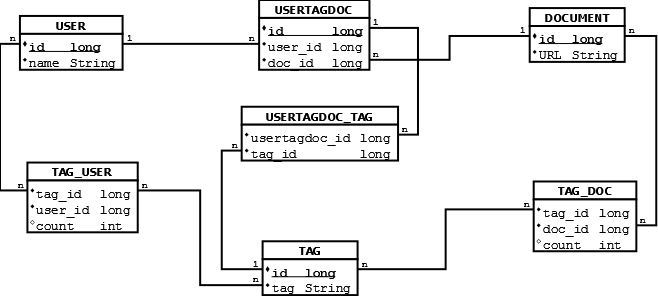
\includegraphics[width=1\textwidth]{db.png}
\caption{Baza danych}
\label{fig:db_fig}
\end{figure}


\subsection*{Opis tabel:}
\begin{itemize}
	\item USER: tabela zawiera dane użytkowników, ich $id$ i unikalną nazwę pobraną z serwisu delicous.
	\item DOCUMENT: tabela zawiera dane o dokumentach. $URL$ który reprezentuje dokument jest unikalny. Ponieważ adresy stron po pominięciu ostatniego slasha/backslasha prowadzą do tych samych witryn, przy sprawdzaniu unikalności linku brane pod uwagę są wszystkie kombinacje adresów.
	\item TAG: tabela zawierająca adnotacje stron.
	\item USERTAGDOC i USERTAGDOC\_TAG: są to tabele które służą do zapisania w bazie danych relacji nadania $k$ tagów: $t_n, t_{n+1}, \dots, t_{n+k}$ przez użytkownika $user_j$  dokumentowi $doc_m$. Dodatkowo wartość $k$: ilość przypisanych tagów, zapisana jest w polu $count$ tabeli USERTAGDOC.
	\item TAG\_USER i TAG\_DOC: tabele zawierające redundantne dane przyśpieszające wykonywanie innych operacji. TAG\_USER zwiera informacje o ilości dokumentów opisanym tagiem $tag_k$ przez użytkownika $user_n$. Druga tabela zawiera informacje o liczbie przypisań tagu $tag_k$ do dokumentu $doc_m$. Tabele te są wykorzystywane głównie dla szybszego zbierania danych dla algorytmów Adapter PageRank i SocialPageRank.
\end{itemize}





\section{Interface użytkownika TODO}

TODO: więcej

Interface uzytwkonika napisany jest przy pomocy technologi google-web-toolkit. Użytkownik po wczytaniu zapytaniu i nacisnieciu ENTER otrzymuje wyniki zapytania.

\section{Lucene}

Lucene jest biblioteką napisaną w Javie. Biblioteka ta jest w stanie indeksować dużą ilość dokumentów z różnych źródeł i przeprowadzać wyszukiwania w tych tekstach. W opisywanej aplikacji, framework Lucene przechowuje źródła stron, o których informacje zostały pobrane z serwisu delicous i zapisane w bazie danych. 

\subsection{Pobieranie stron}

W pewnych odstępach czasu, wątek odpowiedzialny za indeksowanie stron sprawdza czy w bazie danych tabela DOCUMENT nie ma informacji o nowych wpisach. Z bazy danych pobrane są informacje o adresach tych stron. Następnie dla każdego adresu URL zostaje pobrana treść strony na którą wskazuje. Strona WWW następnie zostaje oczyszczona ze znaczników HTML, i przekazane do frameworku lucene do zaindeksowania. Jeśli wszystkie czynności zakończą się powodzeniem, w bazie danych zostaje odnotowana informacja o posiadaniu na dysku danego dokumentu. Rysunek \ref{fig:lucene_index_fig} przedstawiony jest cały proces pobierania i przetwarzania danej strony.

\begin{figure}[htb]

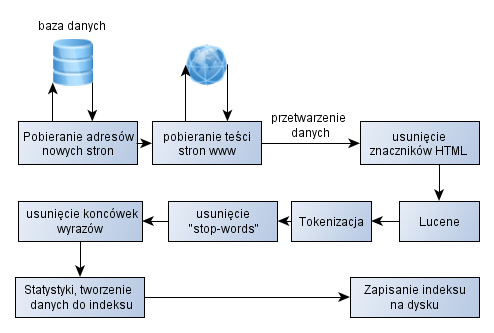
\includegraphics[width=1\textwidth]{lucene_indeksing.png}
\caption{Lucene: pobieranie danych i indeksowanie}
\label{fig:lucene_index_fig}
\end{figure}

Do Lucene zapisywane są następujące informacje: identyfikator $id$ dokumentu z bazy danych, oraz przetworzony tekst strony WWW. Przechowywanie identyfikatora dokumentu w danych Lucene pozwala późniejsze powiązanie wyników wyszukiwania z odpowiednim rekordem w bazie danych. 

W czasie indeksowania biblioteka Lucene wykonuje wiele czynności które pozwalają jej później szybko wyszukiwać informację. Główne z nich to:
\begin{itemize}
\item Tekst zostanje przetworzony na ciąg termów,
\item usunięcie końcówek wyrazów,
\item usunięcie 'stop-words' z tekstu, czyli słów nie mających dużego znaczenia przy wynikach wyszukiwania,
\item obliczenie statystyk, np: wystąpienia słów w dokumencie, odległości od siebie
\end{itemize}

\subsection{Wyszukiwanie}

Czas wyszukiwania zapytania w dokumentach przechowywanych Lucene jest szybkie. Przy małej, poniżej 1GB danych, wyszukiwanie następuje praktycznie w czasie rzeczywistym. Zapytanie jest przekazywane do frameworku, w którym jest one przekształcane na termy. Dla zapytania $q$ i dla każdego dokumentu $d$ wyliczana jest wartość funkcji $score(q,d)$. Wynikiem są dokumenty posortowane wg. wyniku tej funkcji.

$score(q,d) =   coord(q,d)  *  queryNorm(q) * \sum_{t \text{ in } q}  \bigg( tf(t\text{ in } d)  *  idf(t)^2  *  getBoost(t) *  norm(t,d) )$

gdzie:
\begin{itemize}
	\item coord(q,d): funkcja zwraca wartości zależne od miejsca wystąpowania i odległości od siebie szukanych termów w dokumencie.
	\item queryNorm(q): funkcja normalizująca wyniki zapytania
	\item tf(t in d): funkcja wyliczająca częstość występowania danego termu w dokumencie
	\item idf(t) : funkcja wyliczająca częstość występowania termu we wszystkich dokumentach.
	\item getBoost(t) - Lucene pozwala na zwiększenie wagi niektórych termów. Nieużywane w tej aplikacji.
\end{itemize}

Lucene ocenia dokumenty głównie na podstawie funkcji TF-IDF. Każdy dokument reprezentowany jest przez wektor, składający się z wag słów występujących w tym dokumencie. TFIDF informuje o częstości wystąpienia termów uwzględniając jednocześnie odpowiednie wyważenie znaczenia lokalnego termu i jego znaczenia w kontekście pełnej kolekcji dokumentów.

\section{Wyszukiwanie TODO}

$score\_all(doc, q) = \alpha * lucene\_score(doc, q) + \beta * social\_page\_rank\_score(doc) + \gamma * adapt\_page\_rank(doc) + \eta * social\_rank(doc)$

gdzie:

\begin{itemize}
\item $\alpha, \beta, \gamma, \eta$ wspolczynniki wag dla poszczególnych algorytmów
\item $lucene\_score$ - rank dokumentu $doc$ dla zapytania $q$. Zwracane przez framework lucene.
\item $social\_page\_rank$ wynik algorytmu social page rank dla dokumentu $doc$
\item $adapt\_page\_rank$ wynik algorytmu adapted page rank
\item $social\_rank$ wynik algorytmu social rank, działającego na danych pobranych z serwisu digg/twitter/facebook
\end{itemize}

\begin{figure}[htb]

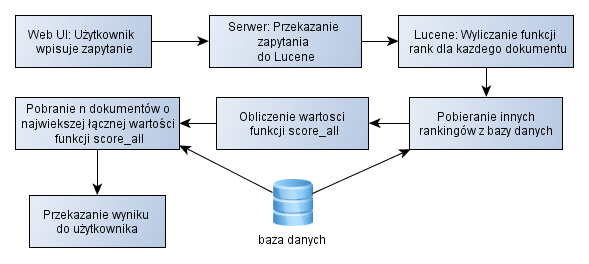
\includegraphics[width=1\textwidth]{search.png}
\caption{Proces wyszukiwania dokumentów i wyliczania ich rank}
\label{fig:search_fig}
\end{figure}

